\chapter{绪论}
\label{chap:introduction}

\section{研究背景及现实意义}
\subsection{医学影像分析的研究背景}

临床医学历经几百年的发展,传统的“视、触、叩、听”已经不能满足现代化医疗的诊断需求,医学影像极大地变革了传统的诊疗体系,成熟的成像模式不断完善,新技术不断涌现,在疾病筛查、早期诊断、治疗方案选择和预后评估等方面发挥着举足轻重的作用。用于医疗诊断的影像使医生能够更早地发现疾病并改善患者预后,介入或术中成像有助于消除和治愈许多检测到的疾病,能更早更有效地诊断身心健康状况,为临床诊疗提供了全面的视角和丰富的信息,迅速地被广泛应用于临床领域。目前临床医学已经无法离开医学影像,并且随着医学影像的发展,临床诊疗将越来越依赖于影像。

在医学成像中,疾病的准确诊断和评估取决于准确的图像采集和图像解释。近年来随着大数据和计算机通讯技术的发展,影像归档和通信系统(Picture Archiving and Communication Systems,PACS)和医学数字成像和通信标准(Digital Imaging and Communications in Medicine,DICOM)等技术的成熟既解决了影像的采集问题,又解决了数据的传输和存储问题。医学影像自1895年伦琴发现X射线以来,综合利用物理中的各种物质波、光电子技术以及计算机技术,从宏观到微观,由静态到动态,由单模到多模,由2D到3D,形成了各种的成像模式包括X射线、超声、计算机断层扫描(Computed Tomography, CT)、磁共振成像(Magnetic Resonance Imaging, MRI)、正电子断层扫描、以及内窥镜和病理切片图像等。

然而,图像解读过程最近才开始受益于不断提升的计算机技术。一旦将医学图像扫描加载到计算机中,研究人员就致力于构建自动化分析系统。早期医学影像分析是通过处理低阶像素(边缘、线)和数学建模(拟合线,圆和椭圆)并应用复合规则系统解决特定任务。而基于训练数据的监督机器学习在医学影像分析中越来越受欢迎,例如活动形状模型(用于分割),图谱(Atlas)方法(分割和配准)以及特征提取和统计分类器的使用(用于计算机辅助检测和诊断),这种模式识别或机器学习方法现在仍然非常流行,并构成了许多成功的商用医学影像分析系统的基础。

医学影像智能分析从简单的计算机辅助检测(Computer Aid Detection,CAD)发展到如今火热的影像组学(Radiomics)\citep{Lambin2015},它将影像内包含的所有信息提取出来然后进行综合系统化分析。更确切的说,影像组学是采用自动化算法从影像的感兴趣区内提取出大量的特征信息作为研究对象,并进一步采用多样化的统计分析和数据挖掘方法从高通量量信息中提取和剥离出真正起作用的关键信息,最终用于疾病的辅助诊断、分类或分级。

当今世界医疗卫生系统每天都会浪费大量的资源和时间,医学图像的大多数解释都是由医生完成的;然而不同的影像质量和不同的工作流程会导致临床上医生对影像内容的理解具有很大的主观性,不同解译人员之间的巨大差异,容易造成对医学影像内容的错误理解会造成错误诊断,导致很多不必要的额外检查,导致治疗计划的延迟,大大减少了如果早期正确发现的生存率或缓解率。即使对于有经验的临床医生来说,图像内容的精确分析也是具有挑战性和耗时的任务。


\subsection{课题研究意义}

计算机智能化工具,结合机器学习和计算机视觉的人工智能(Artificial Intelligence,AI)算法是促进智能诊断的关键因素,尤其是其代表性方法深度学习,深度学习是有多个处理层的计算模型,能学习具有多层次抽象的数据的表示,不但提高了图像内容理解的准确性,它还在数据分析方面开辟了新的前沿,给许多领域都带来了显著改善,包括语音识别、视觉对象识别、对象检测和许多其它领域,例如药物发现和基因组学等。其能不但改善诊疗以及预后效果,还将作为一个固化已有经验的临床助理,给临床医生的工作方式带来转变,显著提高工作流程效率,而不增加临床医生的负担。

人工智能进入医学影像领域,主要为解决当前医学影像分析面临误诊率高、医师缺口大的问题,其一,如何快速自动准确的分析日益增长的医疗影像设备所产生的具有医学分析和指导价值的结构化和非结构化的海量数据。同时由于标准的数据和规范的标注是医疗人工智能发展的前提,反过来,人工智能可以推动医疗数据的标准化建设。其中结构类影像,比如X光、CT,能够非常直观地观察生理结构,判断是否有物理变化的病变,基于人工智能算法实现图像中解剖结构的准确分类和定位是的全自动诊断的基础。而功能类影像能够研究器官对某种物质的代谢能力,从而反映该器官功能,其缺点是不能自主定位异常,不能直接反映真实生理结构,只能通过影像像素和内容综合理解程度来分析代谢的强弱程度,不能实现具有统计学意义的定量分析,诊断结果只能全凭医生的肉眼和经验来判断,导致较高的误诊漏诊率。若结合人工智能算法在定量、定位、精准量化的基础上,通过与正常数据进行统计比对,大大提高了对病变分析的深度,在实现自动辅助诊断上就具备了现实意义。

其二,有经验的医师缺口大,成长曲线陡峭,医师数量增长远不及影像数据增长,在短时间内理解影像数据给出准确诊断的压力会越来越大,远超负荷。AI算法未来可以比专业人员更快,更准确地提取大量数据,挖掘模式和预测,加强疾病诊断,提供治疗计划。突破主要来自AI领域的深度学习方法,其模拟更高层次抽象并决定了高维特征空间中的最佳决策边界,对某些疾病的影像诊断水平已能达到专家水准,同时通过对深度学习理论的研究人工智能的决策机制,未来或为实现精准诊疗、智慧医疗和保障大众健康带来突破性进展。这对于提升基层医疗服务水平、助推分级诊疗将具有重大意义。

总而言之,结合计算机视觉和深度学习算法,能提升医学图像分析领域模式识别的能力,从解剖结构到疾病,让计算机系统能够自主学习经验数据,不仅能更帮助患者更快速地完成健康检查,同时也可以帮助影像医生减少阅片时间,提升效率,降低误诊的概率,既能为经验不足的医生提供辅助决策建议,也能帮助专家节约时间。   

\section{国内外研究现状}

\subsection{图像内容理解的研究现状}

医学影像分析主要涉及图像的内容理解,而实现图像的内容理解是计算机视觉的终极目标\citep{Cootes2004}。可根据研究对象和目标分成低-中-高三层。底层问题主要是针对图像本身及其内在属性的分析,依据灰度值进一步推断物体的几何结构,常见内容有去噪,滤波和特征增强。高层问题主要是针对图像内容的理解和认知层面的,如识别与分割图像中的特定物体与其行为;场景理解和行为推断。中层介于两者之间,着重于不同层级的特征表示。

计算机视觉的起源可以追溯到1966年,以明斯基布置让学生构造一个视觉系统的暑期项目为起点,早期研究主要集中于底层视觉信息处理。
Marr\citep{Marr1982Vision}定义了计算机视觉研究的三个层次,自底向上(bottom-up)的分成表达、算法、和实现,将视觉描述为从二维视觉阵列(在视网膜上)到三维描述世界输出的多层表达,从基本简约图(Primal Sketch),到2.5D深度简约图,再到3D模型,如图\ref{fig:ch01_01},希望先把三维结构从图像里面恢复出来,在此基础上再去做理解和判断。

\begin{figure}[!htbp]
    \centering
    %trim option's parameter order: left bottom right top
    %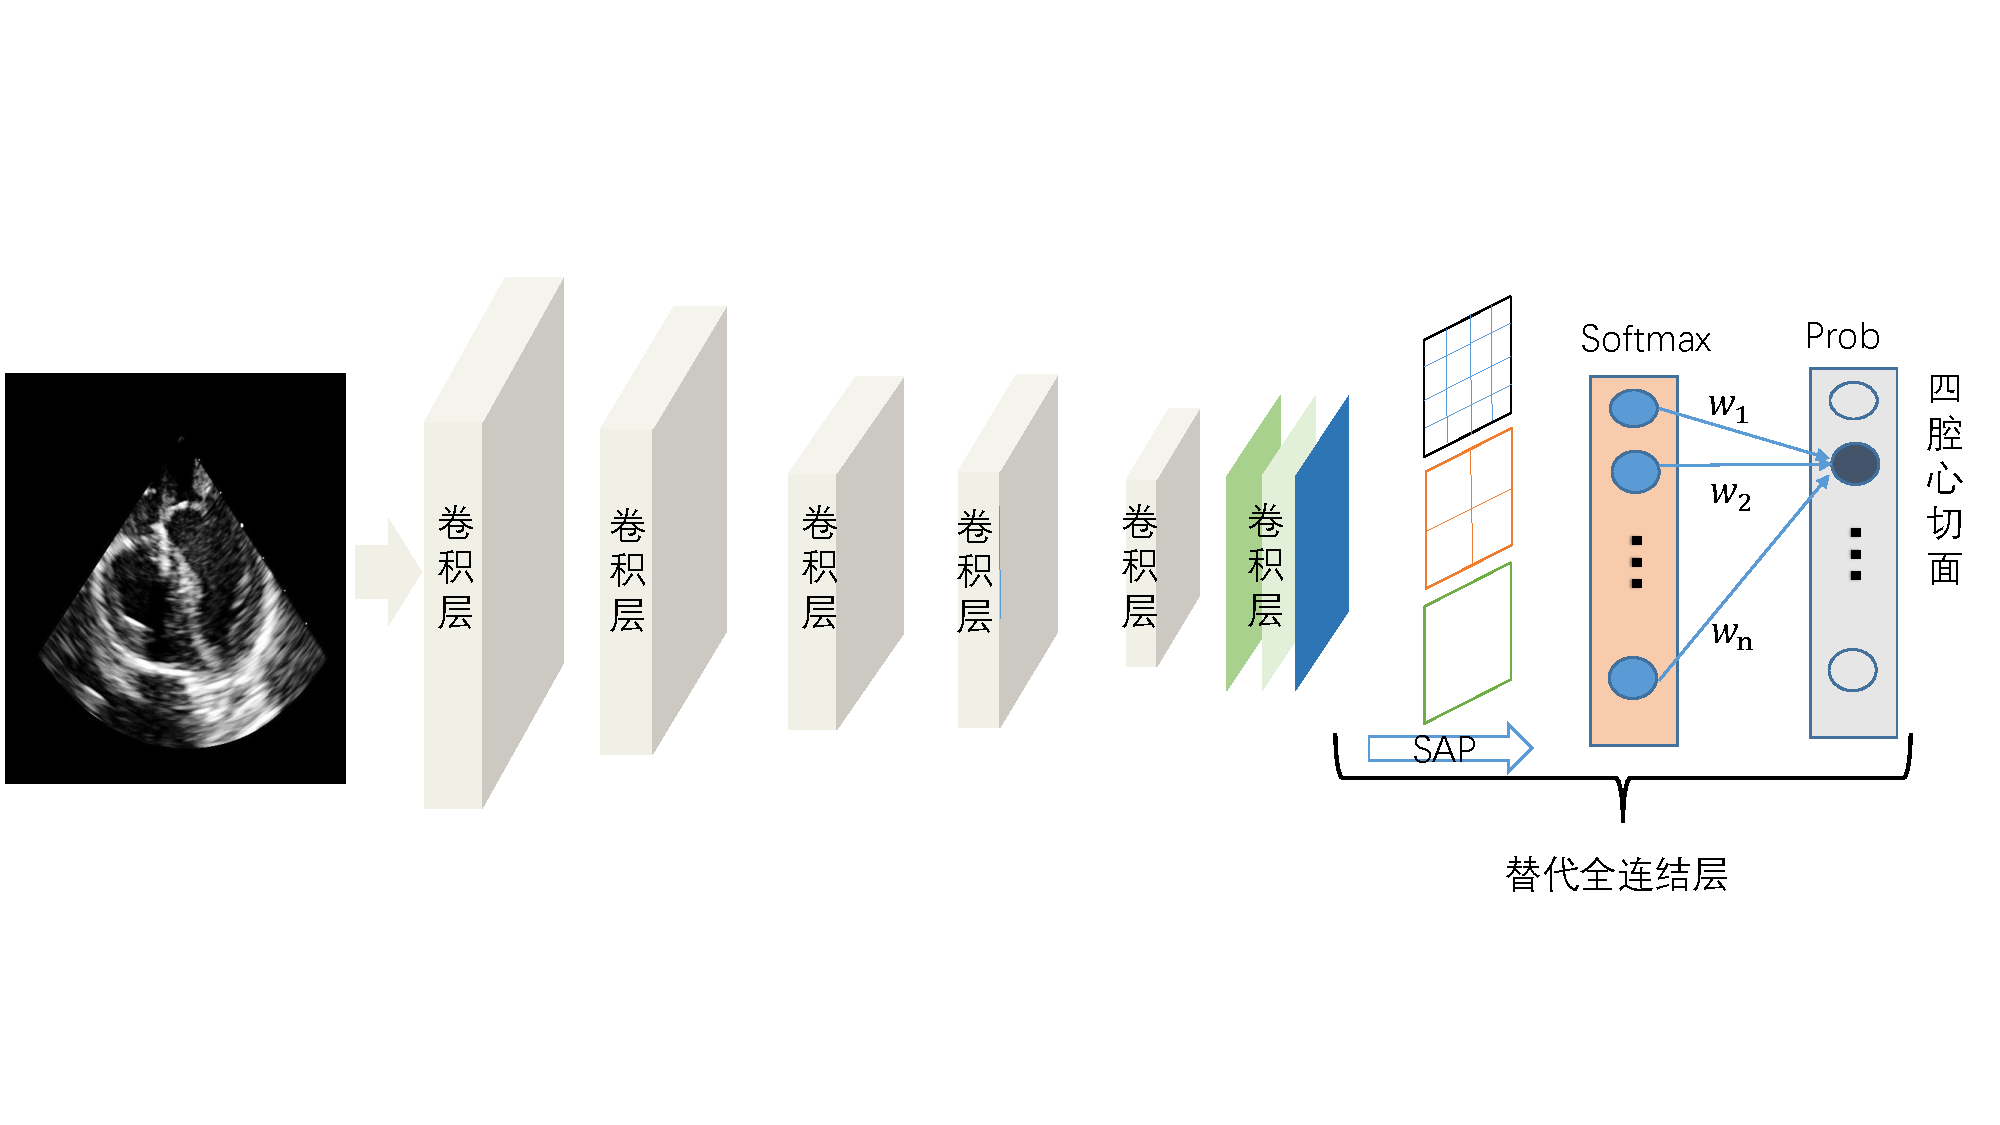
\includegraphics[trim = 30mm 0mm 30mm 0mm, clip, width=0.45\textwidth]{ch03_02}
    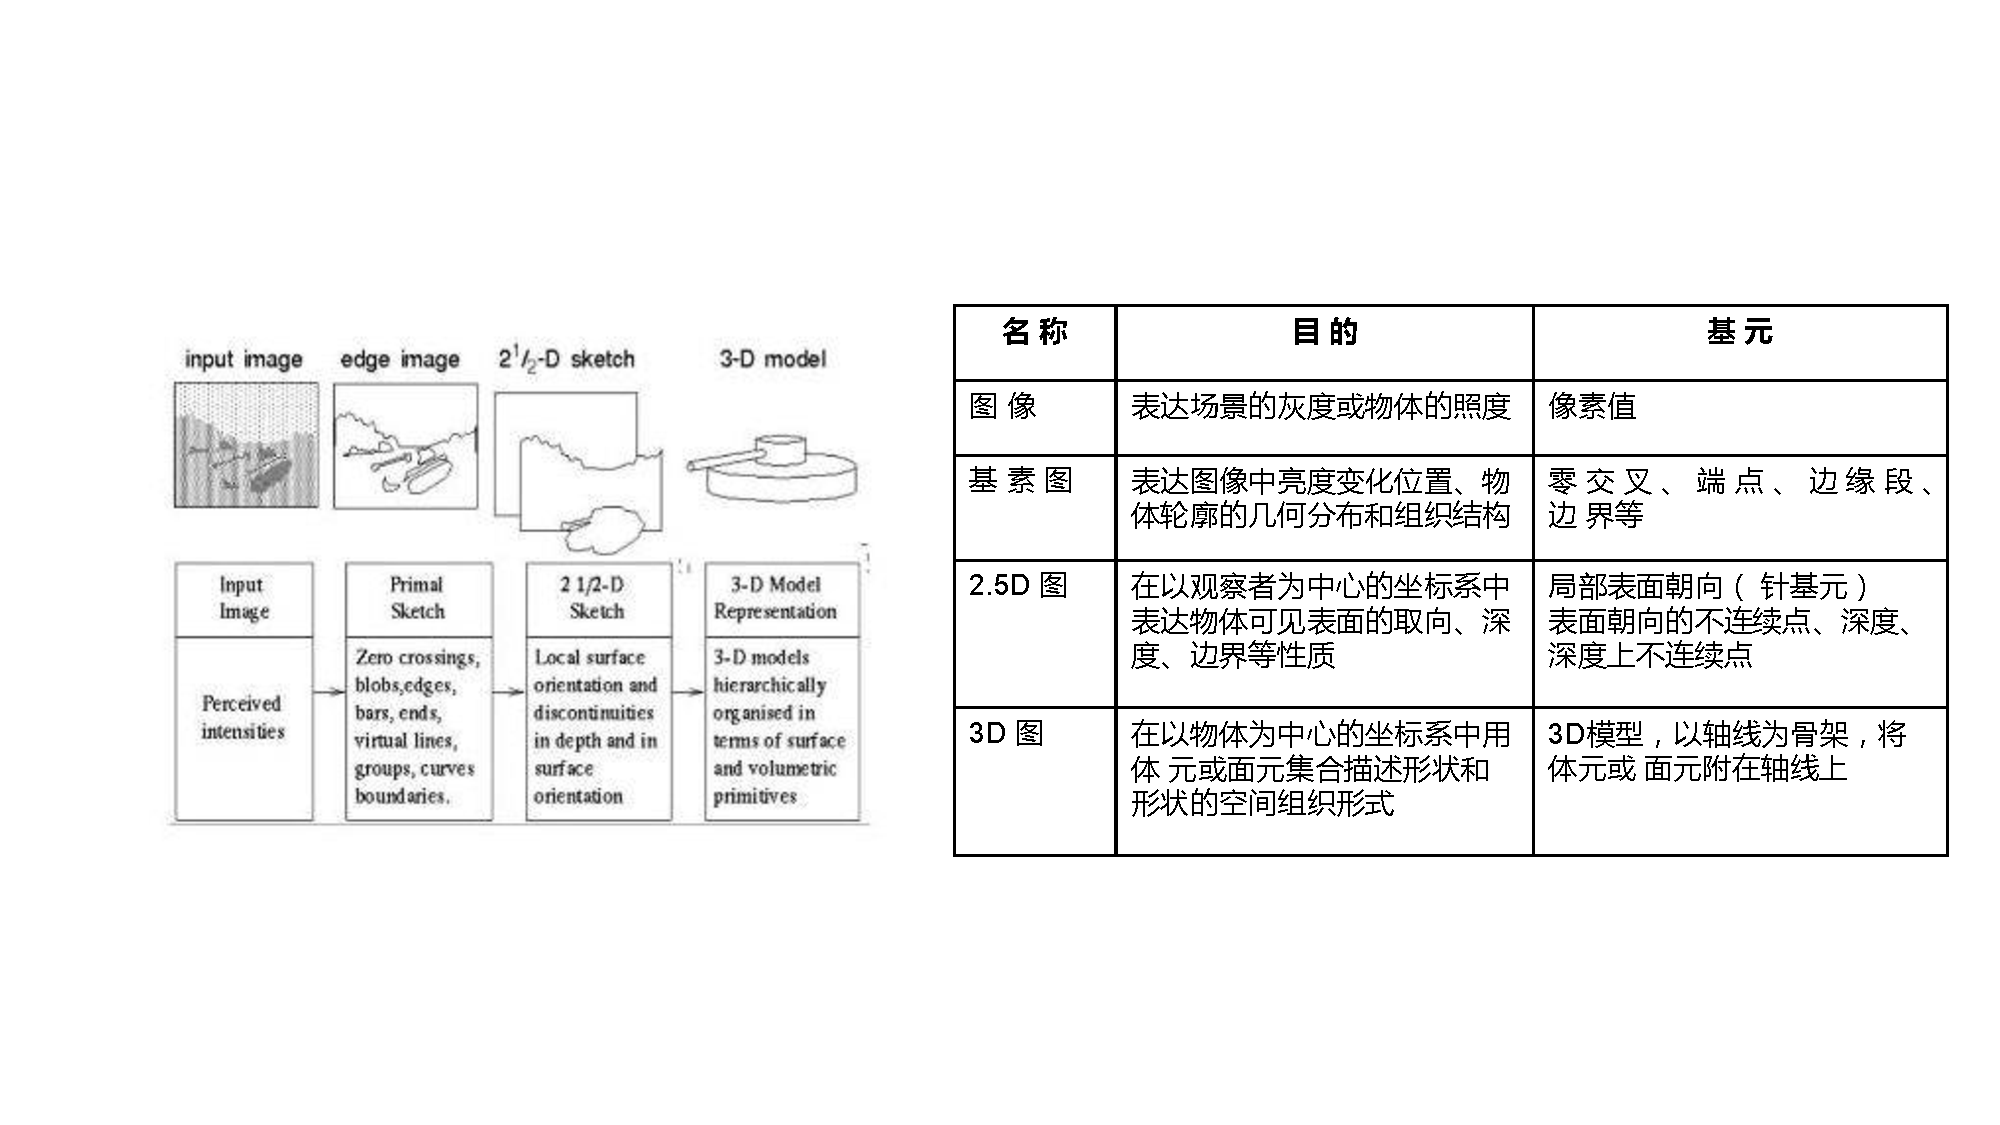
\includegraphics[width=0.9\textwidth]{ch01_01}
    \caption{David Marr视觉计算理论的分层结构示意图}
    \label{fig:ch01_01}
\end{figure}

从20世纪80年代开始,基于逻辑学和知识库推理的专家推理系统在人工智能领域大行其道,计算机视觉的理论方法论随之改变,Biederman在Marr的基础上提出组成识别理论(Recognition by Component Theory)。该理论认为通过把复杂对象解译(Image Parsing)为简单的部件形状,就可进行视觉统计模式匹配。Treisman等\citep{treisman1980a}提出特征融合理论(Feature Intergration), 认为视觉处理是一个以自下而上、局部交互作用的过程。Itti等\citep{Itti2005}提出适用于自然图像的高斯金字塔视觉注意机制模型模型。研究发现要让计算机理解图像,不一定先要恢复物体的三维结构。利用包括统计形变模型\citep{Cootes2004}以及能量泛函模型\citep{Kass1988},对图像进行解译(Image Parsing),将物体形状、颜色和纹理等先验特征进行统计模式匹配,寻找一个层次化、结构化的解释是计算视觉的核心问题。

\begin{figure}[!htbp]
    \centering
    %trim option's parameter order: left bottom right top
    %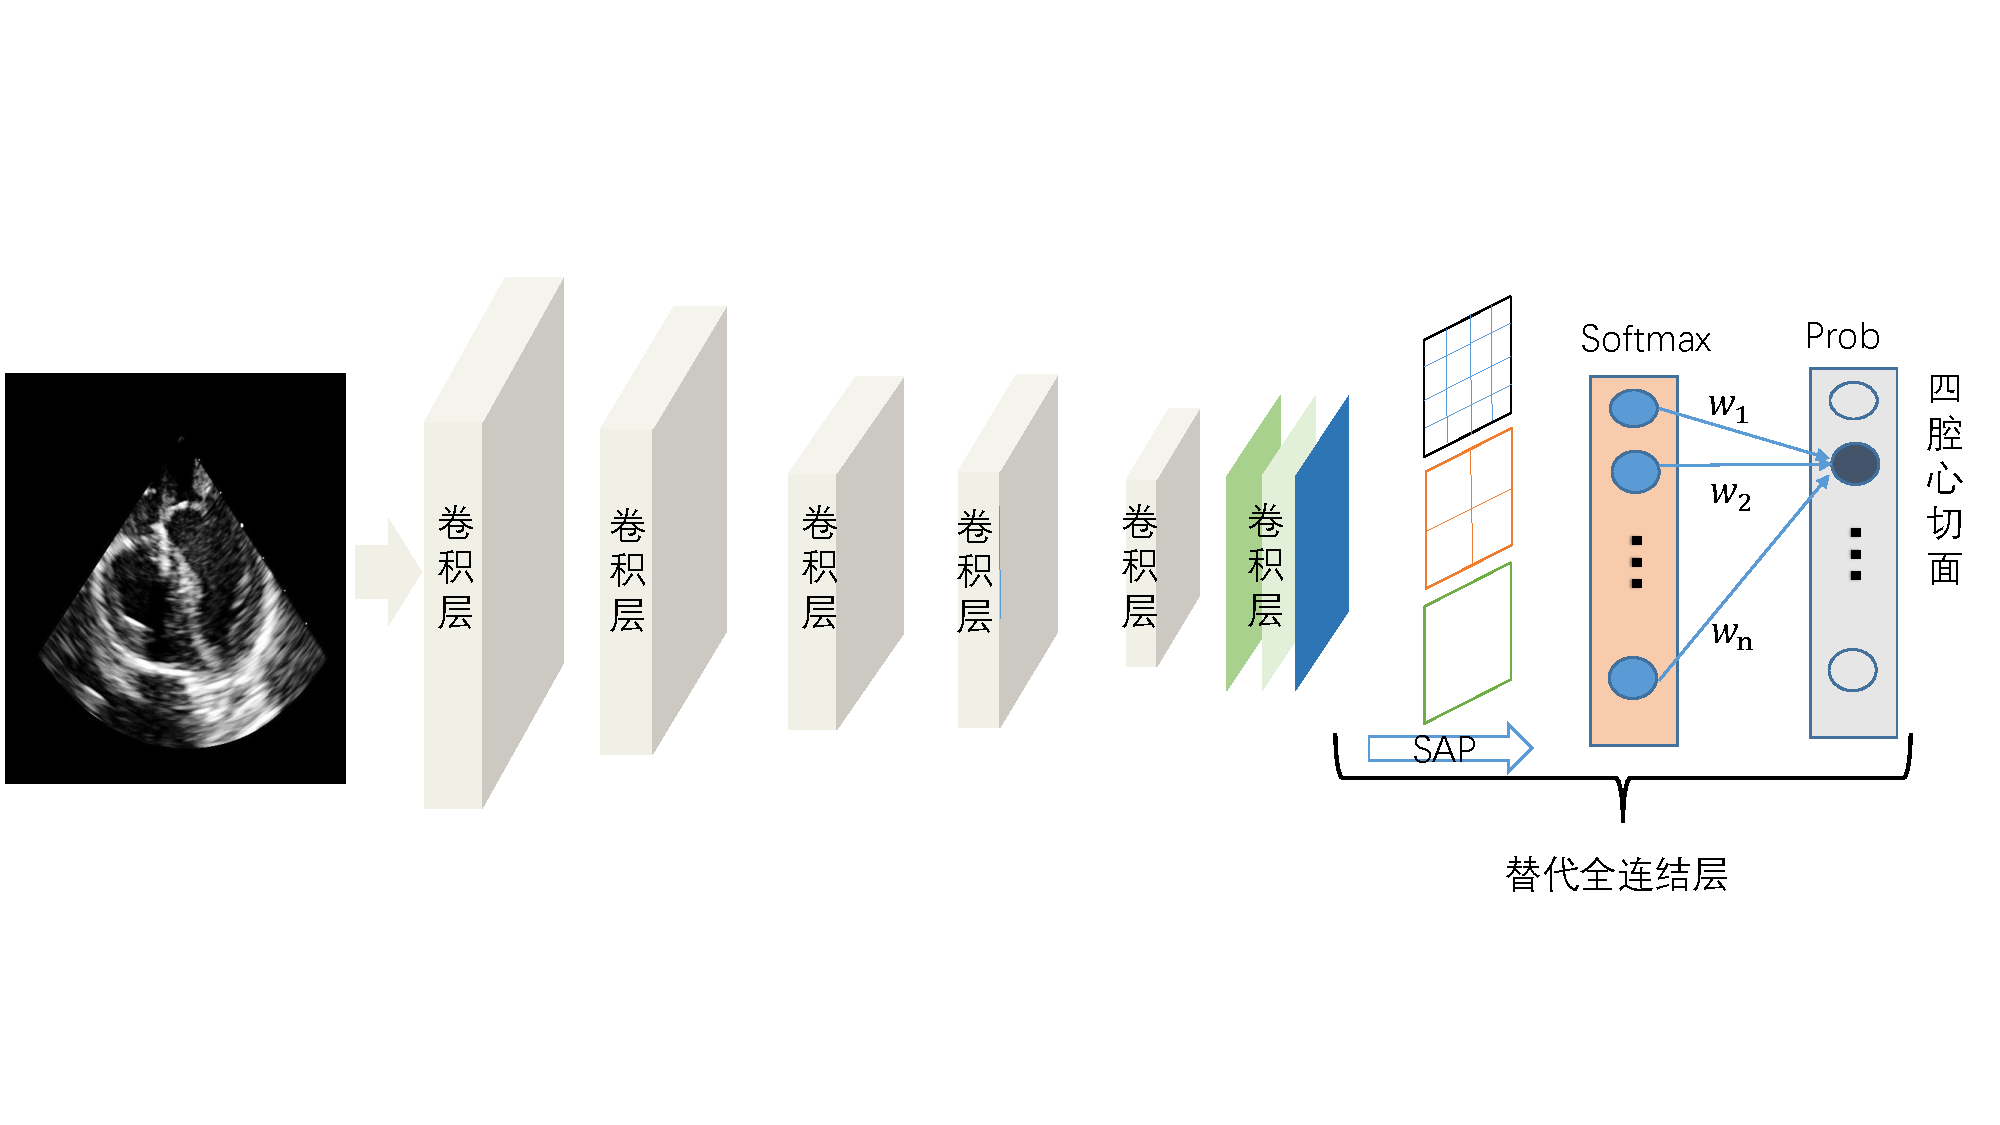
\includegraphics[trim = 30mm 0mm 30mm 0mm, clip, width=0.45\textwidth]{ch03_02}
    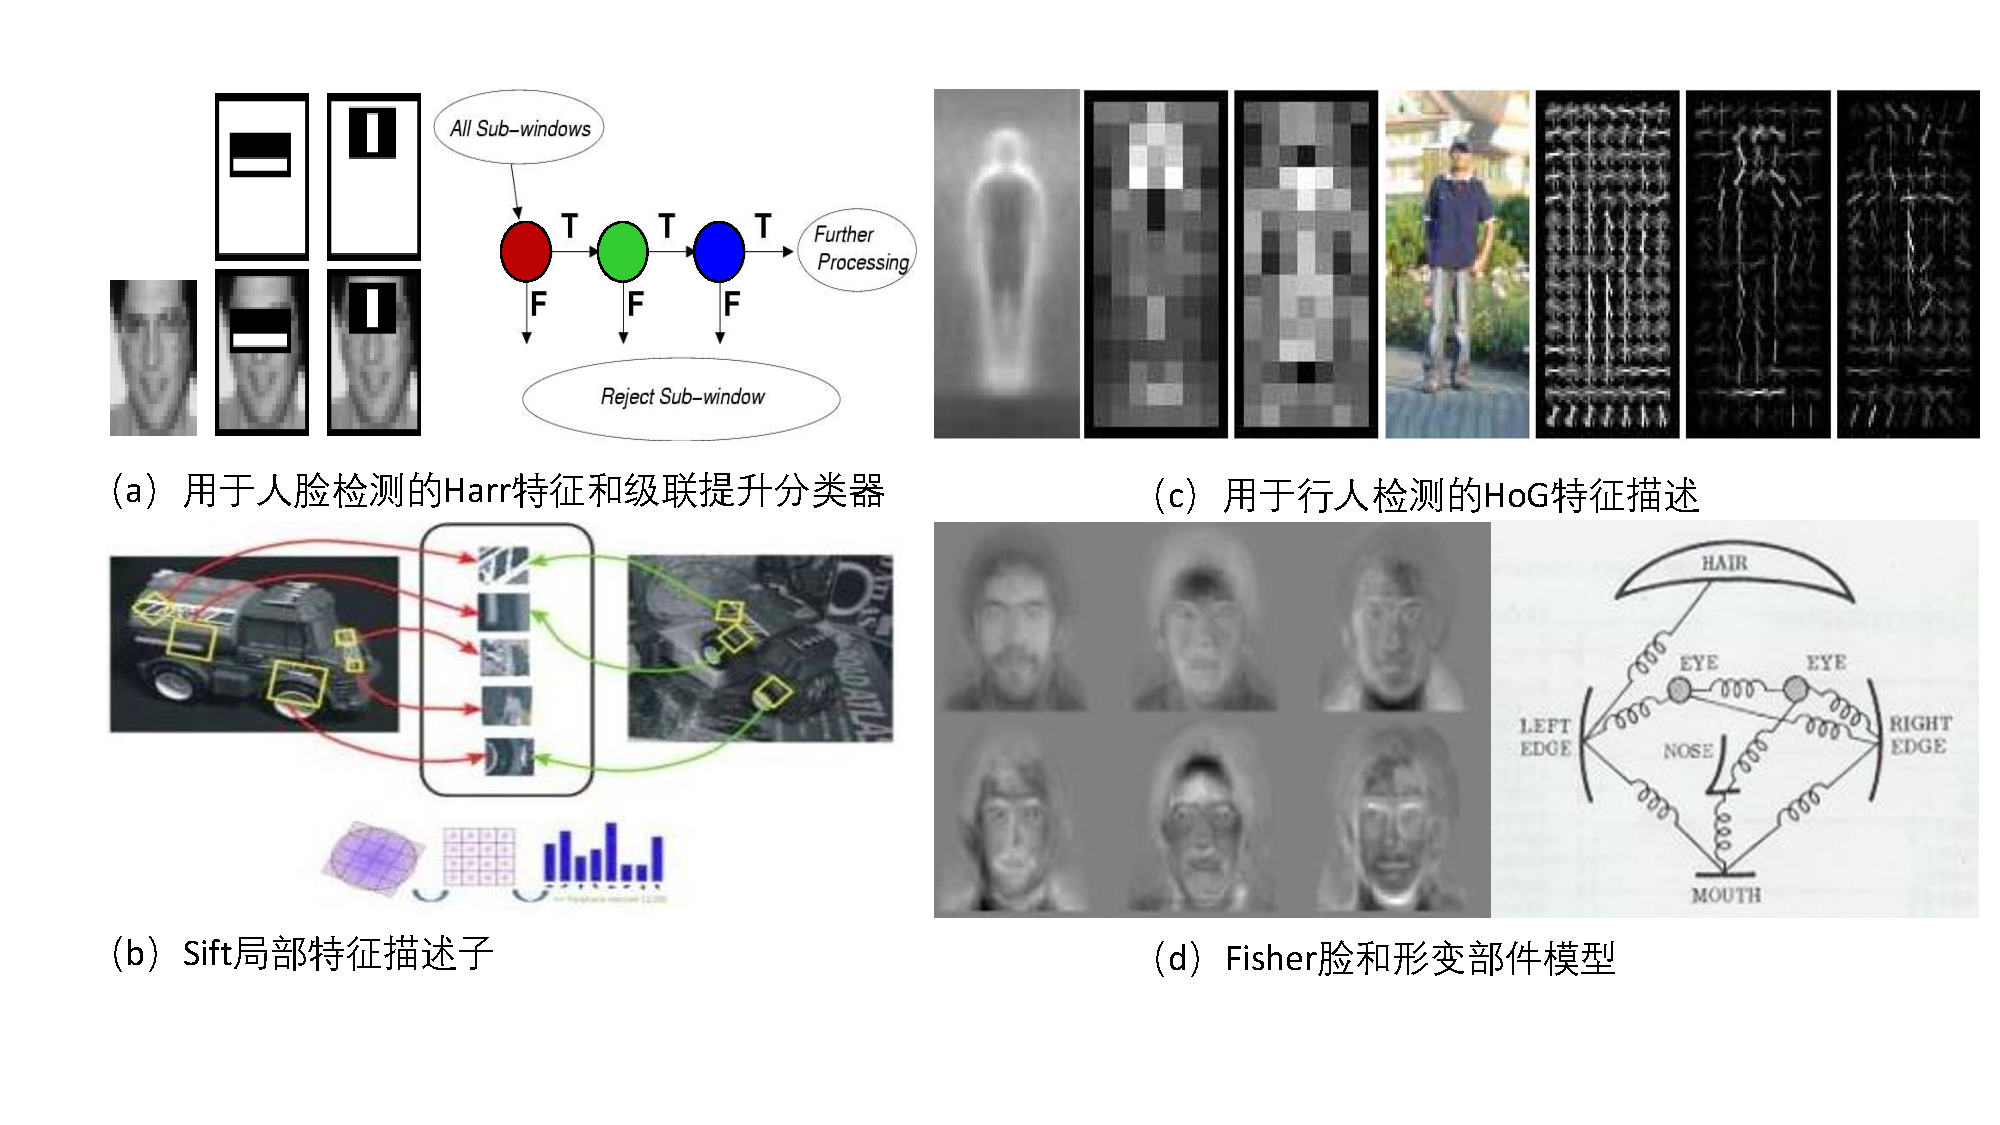
\includegraphics[width=0.9\textwidth]{ch01_02}
    \caption{局部特征结合机器学习的机器视觉代表性方法举例}
    \label{fig:ch01_02}
\end{figure}

进入新世纪后,互联网产生了海量图像数据,大规模数据集也随之出现,导致面向描述符的机器学习方法开始盛行,之前需通过规则、知识或统计模型设计形状、颜色、纹理等先验表征,易受额外影响不具有统计不变性,通过统计手段寻找能够刻画对象最本质的一些局部特征,其进展直接导致诸多应用的出现,如:图像搜索技术进入实用。目标识别领域涌现出空间金字塔(Spatial Pyramids)\citep{Lazebnik2006}、矢量量化(Vector Quantization)\citep{Yang2009b},以及在计算机视觉的各个阶段使用的各种机器学习工具。Lowe\citep{Lowe2004}提出旋转和尺度不变的局部特征描述符( Scale Inrariant Feature Transform,SIFT),改进后成为模式识别中的经典模型。Viola和Jones\citep{Viola2001}提出基于哈尔特征和级联Adaboost分类器人脸检测框架;Grauman等\citep{Grauman2005}发展了词袋模型(Bag of Word,Bow)用于图像物体识别;Dala等\citep{Dalal2005}提出方向梯度直方图(Hog)特征,利用变形部件模型结合支持向量机进行行人检测。因此,从完全由人类设计的系统转变为由使用计算机提取示例数据进行训练获得特征向量的的系统,计算机算法决定了高维特征空间中的最佳决策边界,设计此类系统的关键步骤是从图像中提取判别特征,该过程仍然是由人类手工设计完成的。

故合理的下一步就是让计算机自动从数据学习最佳特征表示,如图\ref{fig:ch01_03}揭示了手动设计特征的传统方法与自动提取特征的深度学习方法的区别,模型由多层组成,将输入数据转换为输出(例如疾病存在/不存在),同时学习更高层次的特征。目前最成功的图像分析模型是卷积神经网络(convolutional neural networks,CNN),Fukushima早在1980年就提出有关CNN的工作\citep{Fukushima1982Neocognitron}。LeCun等\citep{Lecun1990Handwritten}提出的LeNet是在手写数字识别领域的第一个成功的实际应用。在医学图像处理中,GPU首先被引入用于分割,重建和配准,然后被用于机器学习。但在开发各种新技术以有效地训练深度网络之前,CNN在计算机视觉领域并没太成功。分水岭是Krizhevsky等人\citep{Krizhevsky2012}在2012年12月参加ImageNet\citep{Deng2009ImageNet}识别竞赛挑战做出的贡献,提出AlexNet大幅度(领先10\%)赢得该竞赛。随后,使用相关但更深的架构取得了进一步的进展\citep{Simonyan2014a,Szegedy2015,he15}。在计算机视觉各个任务领域,深度卷积神经网络现在已经成为首要选择的技术。
\begin{figure}[!htbp]
    \centering
    %trim option's parameter order: left bottom right top
    %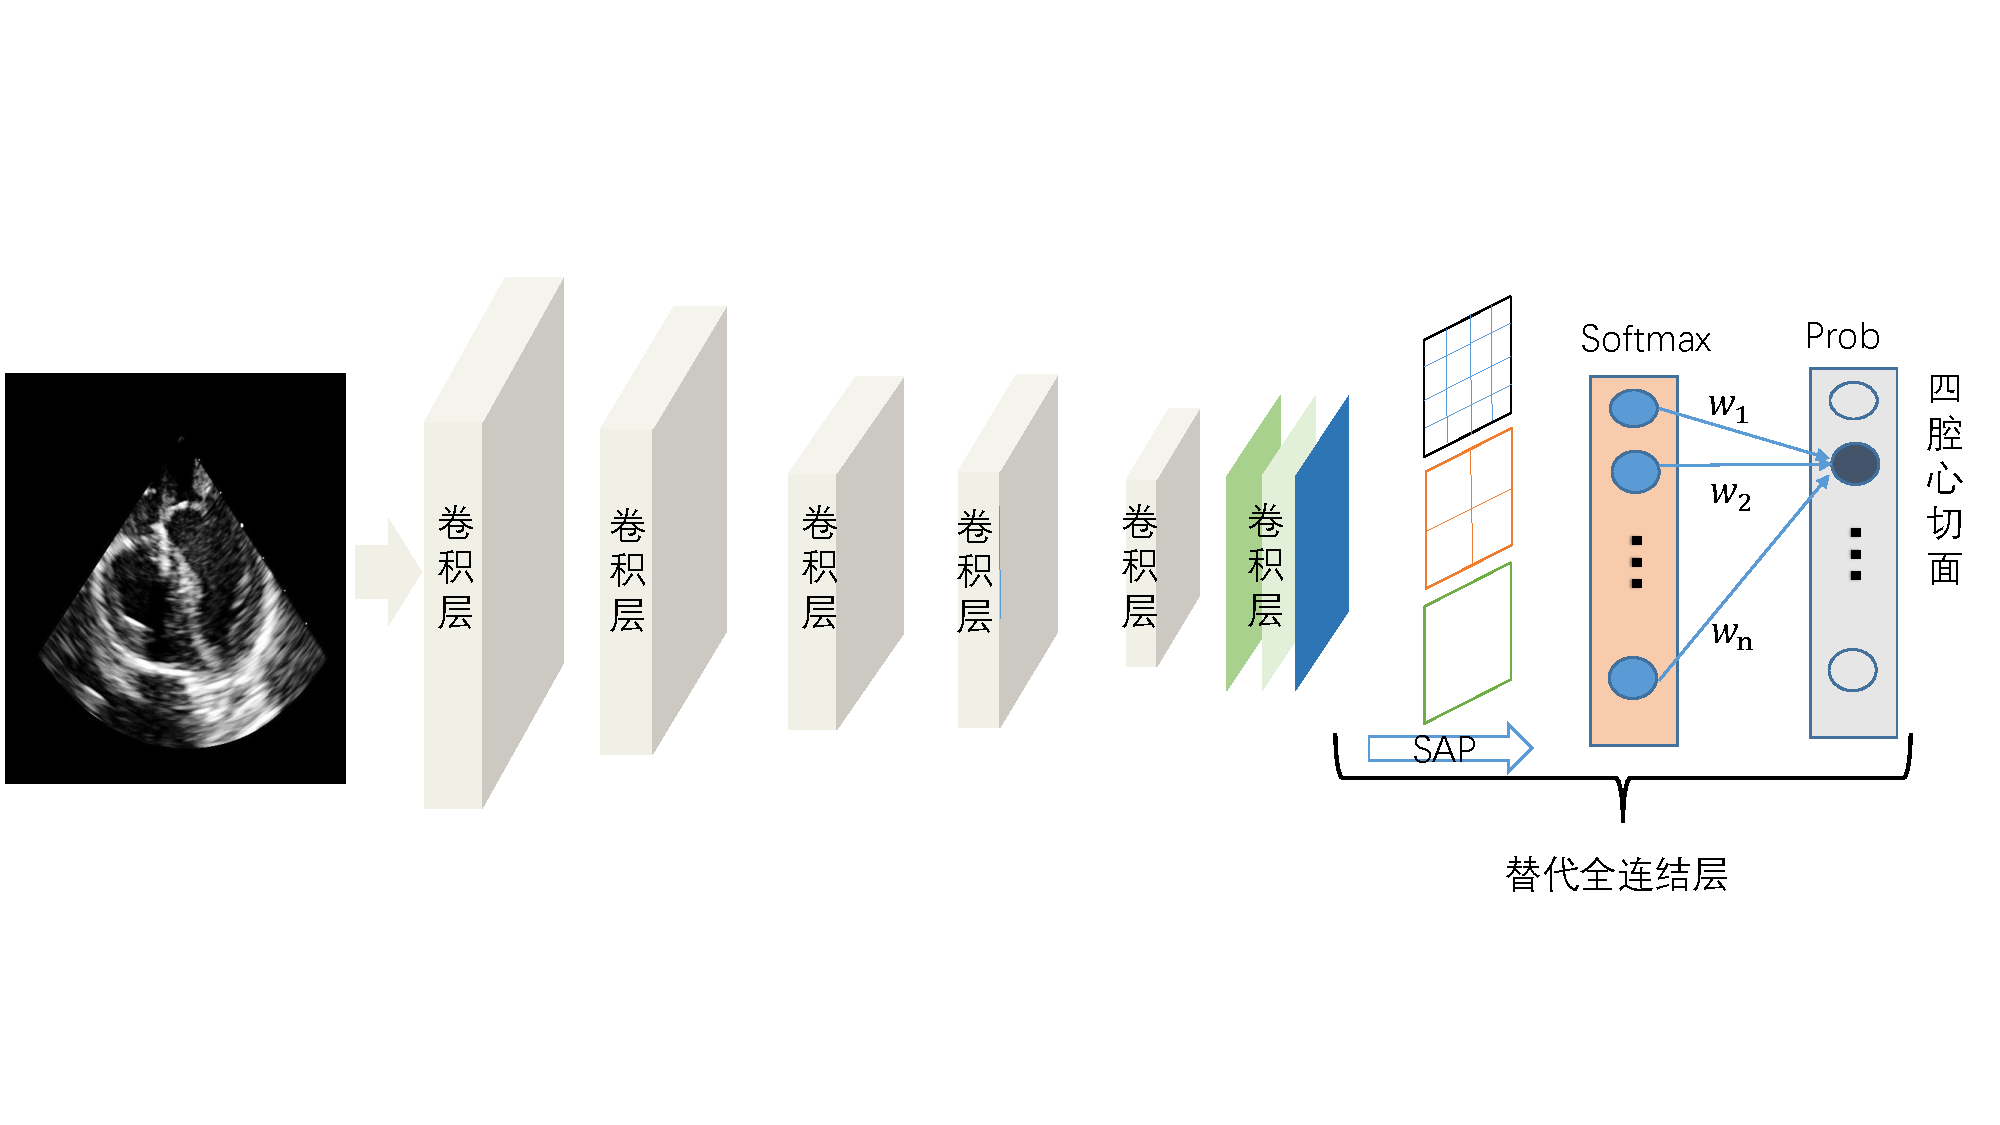
\includegraphics[trim = 30mm 0mm 30mm 0mm, clip, width=0.45\textwidth]{ch03_02}
    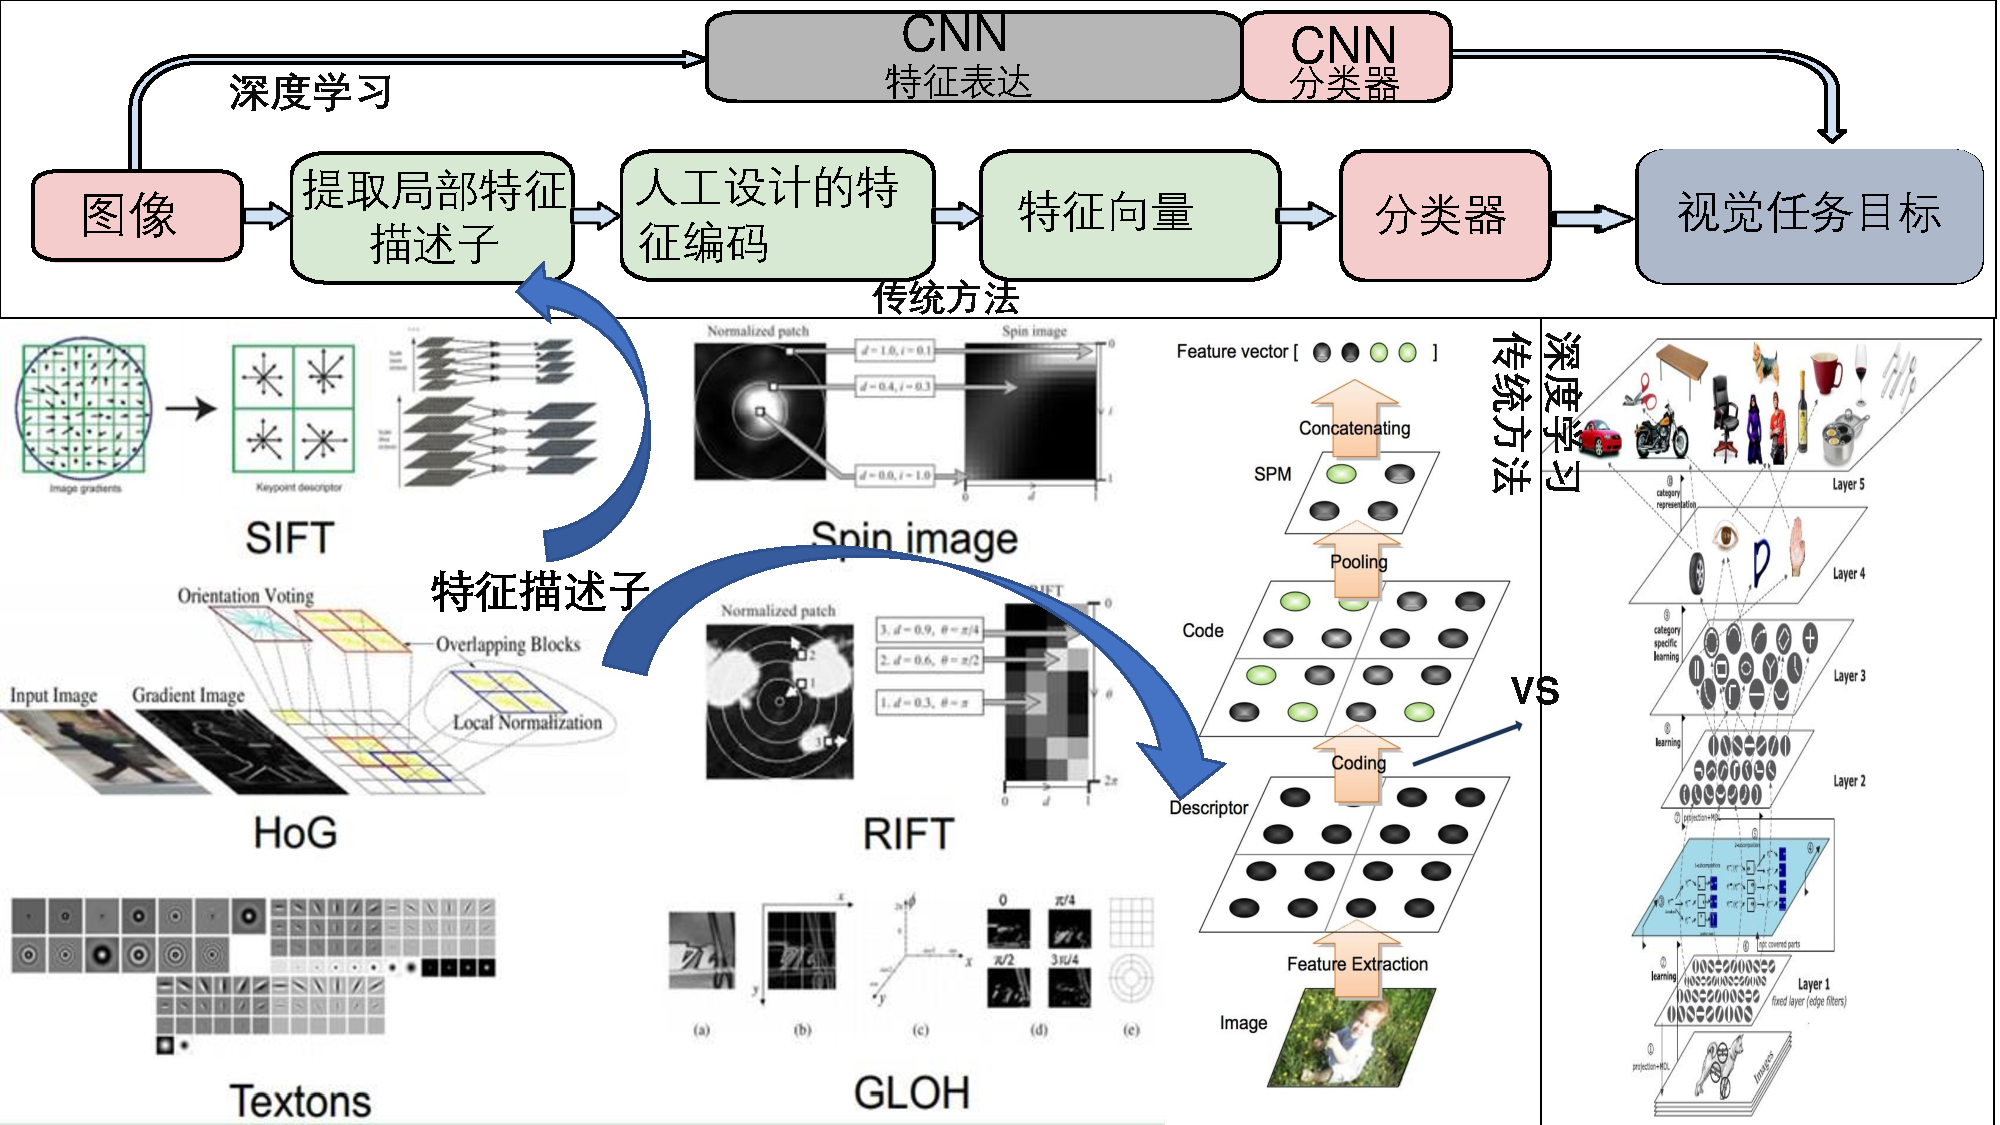
\includegraphics[width=0.9\textwidth]{ch01_03}
    \caption{传统图像识别方法与深度学习方法对比}
    \label{fig:ch01_03}
\end{figure}

另外一些研究者从模拟生物视觉机制出发,通过对感受野、注意机制、颜色特性和光流等方面进行计算机视觉研究。Hubel和Wiesel\citep{Hubel1962Receptive}对猫视觉皮层细胞的信息处理模式做了深入研究,提出视觉感受野(Receptive Field)概念,进一步发现了视觉皮层通路中对于信息的分层处理机制。Riesenhuber等\citep{Riesenhuber1999}首次从生物学的角度上模拟建立分层的视觉处理模型(Hierardical Model and X, HMAX),其模型与文献\citepns{Itti2005}中的模型类似。Berthold等\citep{Horn1981}认为人类感知不是对视网膜上降采样图像的解释,而是对光学排列和流动的直接感受体验,提出光流(Optical Flow)用于描述图像灰度的表面活动形式,即获取运动场得到丰富的场景运动和场景结构等信息。

另外一些研究者从模拟生物视觉认知机制出发,McClelland和Pitts等依据神经元连接方式提出神经细胞模型MP ,相关节点单元(Node)是最小的加工单元,节点之间通过通过兴奋和抑制两种连接方式联结成网络,利用“Hebb规则”的学习机制,指出神经元在不同时刻需具有变化的强度激活值(Activation Value),该理论成为连接主义理论的代表性理论。Rosenblatt等\citep{Rosenblatt1958}提出了由单层神经元组成的感知机(Perceptron)来完成线性分类任务;Fukushima等\citep{Fukushima1982Neocognitron}提出了神经网络多层的结构,但是并没有提出如何学习这个结构;Rumelhar和Hinton等人\citep{Rumelhart1988Learning}根据求导的链式法则提出了反向传播(Backpropagation,BP )算法,解决了多层神经网络所需要的复杂计算量问题。Hopfield提出利用能量函数的概念来研究一类具有固定权值的循环神经网络的稳定性并付诸电路实现。

\begin{figure}[!htbp]
    \centering
    %trim option's parameter order: left bottom right top
    %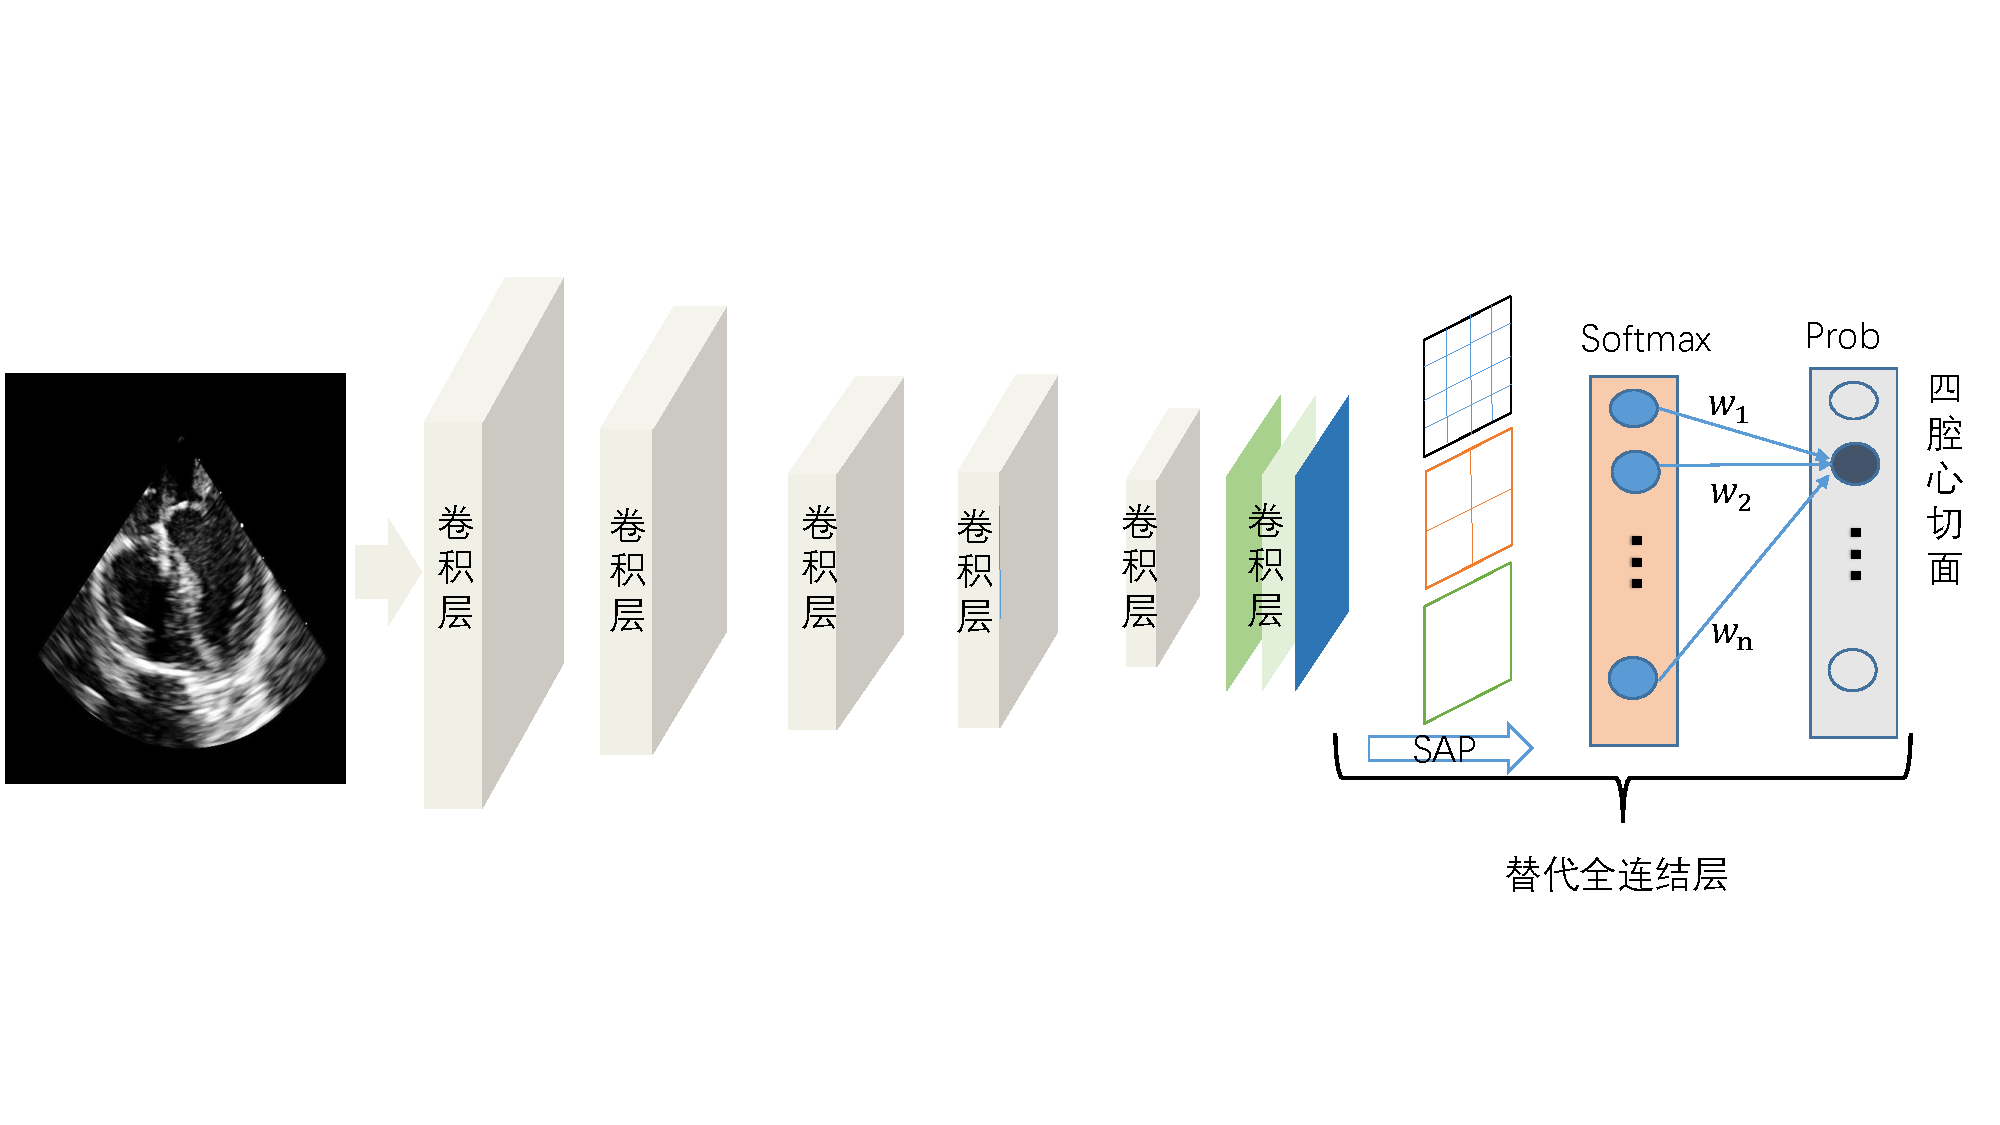
\includegraphics[trim = 30mm 0mm 30mm 0mm, clip, width=0.45\textwidth]{ch03_02}
    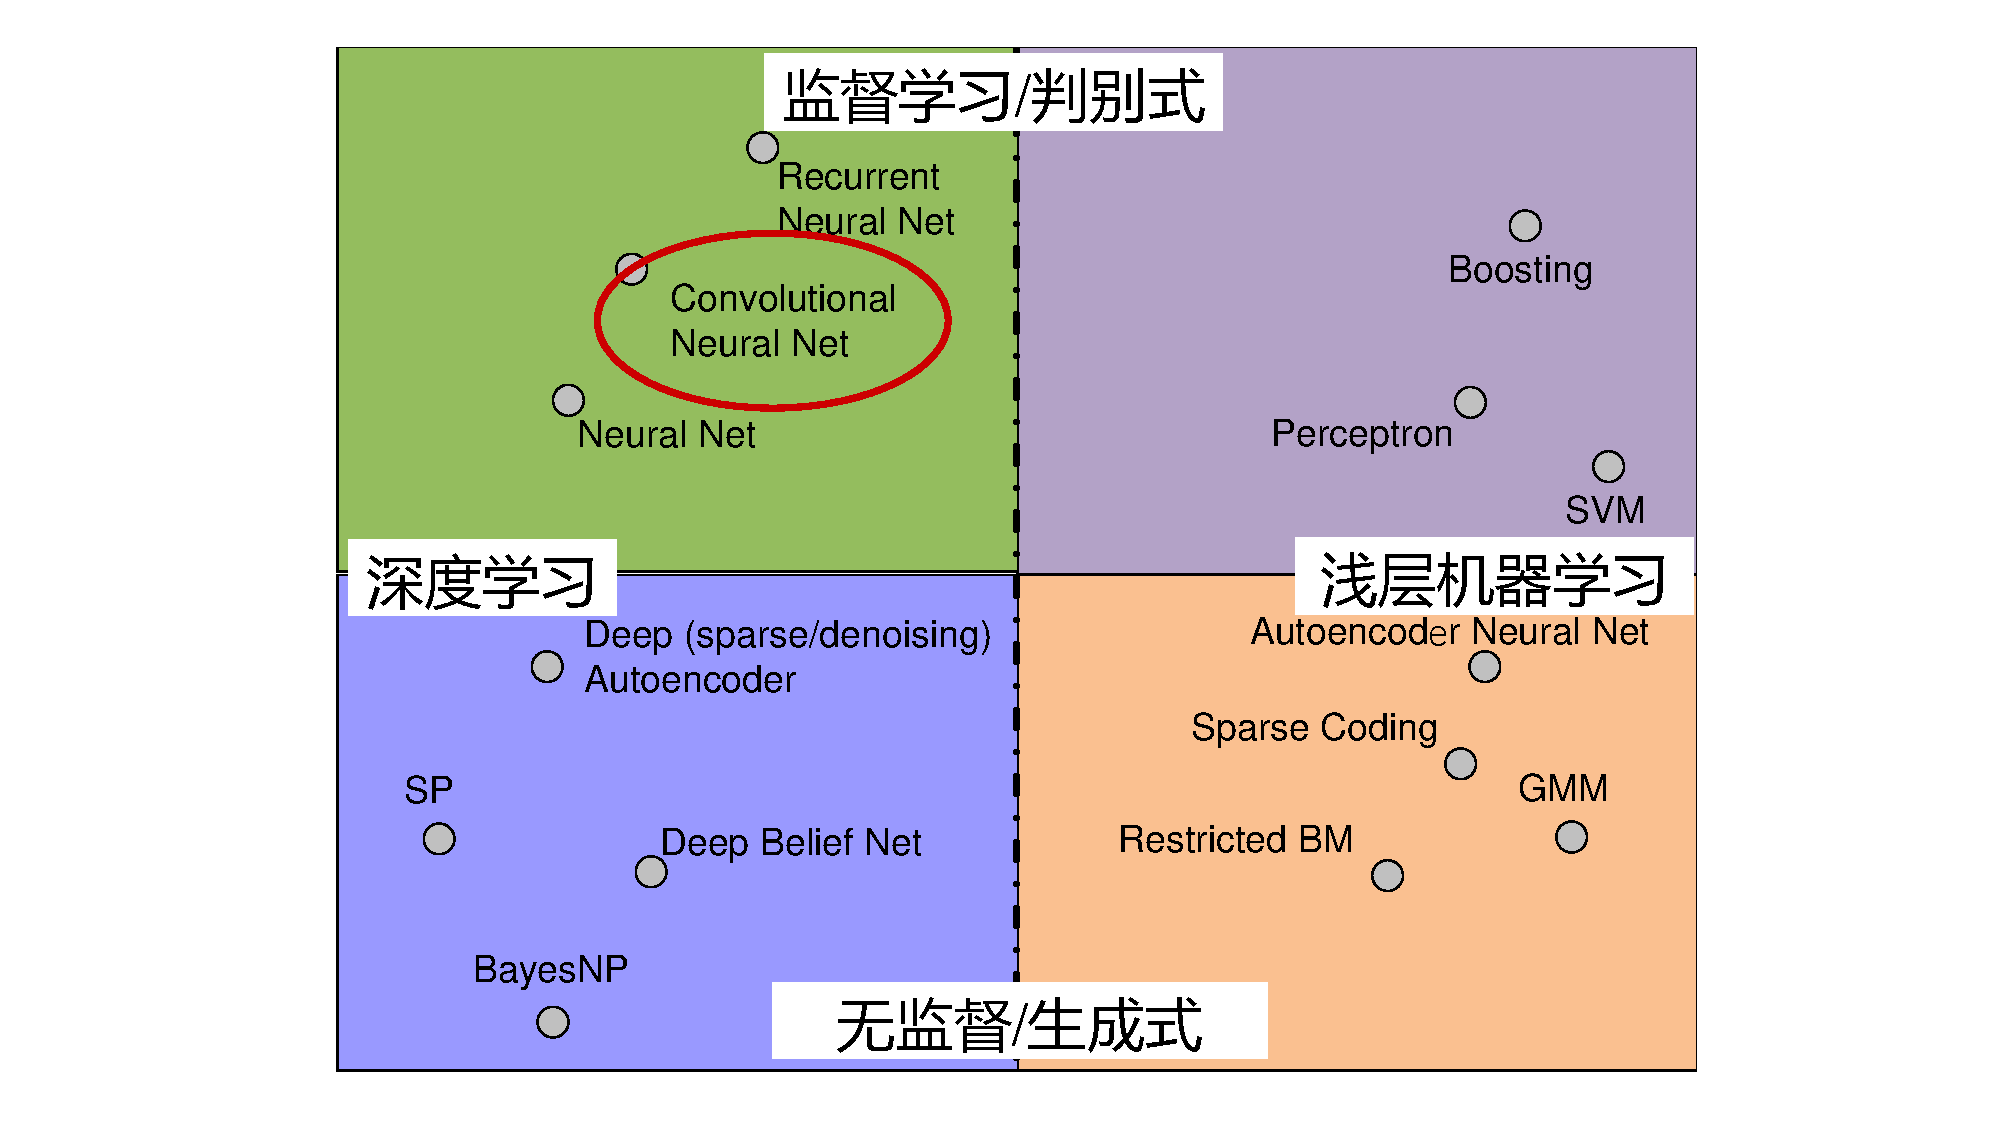
\includegraphics[height=80mm,width=0.9\textwidth]{ch01_04}
    \caption{统计机器学习方法分类总结}
    \label{fig:ch01_04}
\end{figure}

\subsection{深度学习在医学图像分析应用的研究现状}


医学影像分析界业已注意到当前从使用手工设计特征转换到从数据中学习特征的关键进展,在AlexNet突破之前,依据模型结构深浅和监督与非监督四个维度度现有机器学习方法进行归类(如图\ref{fig:ch01_04})。通过对有限样本统计理论、和VC维泛化能力等机器学习理论的研究,相继提出了各种各样的浅层机器学习模型,如支持向量机(Support Vector Machines,SVM)、 集成学习(Boosting)、稀疏编码(Sparse Coding)等,这些模型基本上可视作只有有一层隐层节点(如SVM、Boosting)的浅层神经网络,神经网络和深度学习背后神经科学的基本理念如上节所述。这些模型无论是在理论分析还是实际应用于医学图像分析中都获得了不小的成功,特别是用于检测异常情况,而且还用于分割等相关领域。尽管有这些发展,但检测的假阳性率相对较高。受限于计算力早期的神经网络通常只有几层,由于理论分析的难度大,训练方法又需要很多经验和技巧,这个时期浅层人工神经网络研究反而相对沉寂。

自2006年hiton等\citep{Hinton2006a}提出深度学习以来,方兴未艾的深度学习真正改变了计算机视觉之前的定义,它正在成为计算机视觉领域机器学习工具最优的选择之一。特别是卷积神经网络已被证明是众多计算机视觉任务的强大工具。世界各地的医学图像分析团队正在迅速进入该领域,并将其和其他深度学习方法应用于各种各样的应用,令人鼓舞的结果正不断涌现,如图\ref{fig:ch01_05},从左上到右下依次为:乳房X线图像质量分类\citep{Sickles2006Use},大脑病灶分割(\citep{Abr2016Improved}),气道树分割中的泄漏检测 \citep{Charbonnier2016Improving},视网膜病变分类(Kaggle糖尿病视网膜病变图像)\citep{Grinsven2016Fast},前列腺分割,结节分型,淋巴结中的乳腺癌转移检测,皮肤病变分类\citep{Esteva2017Dermatologist}和来自Yang等人\citep{Yang2016Cascade}的X射线骨骼抑制技术。文献\citep{Litjens2017Asurvey,Shen2017a,Greenspan2016}对深度学习应用于医学图像分析做了专门综述。

\begin{figure}[!htbp]
    \centering
    %trim option's parameter order: left bottom right top
    %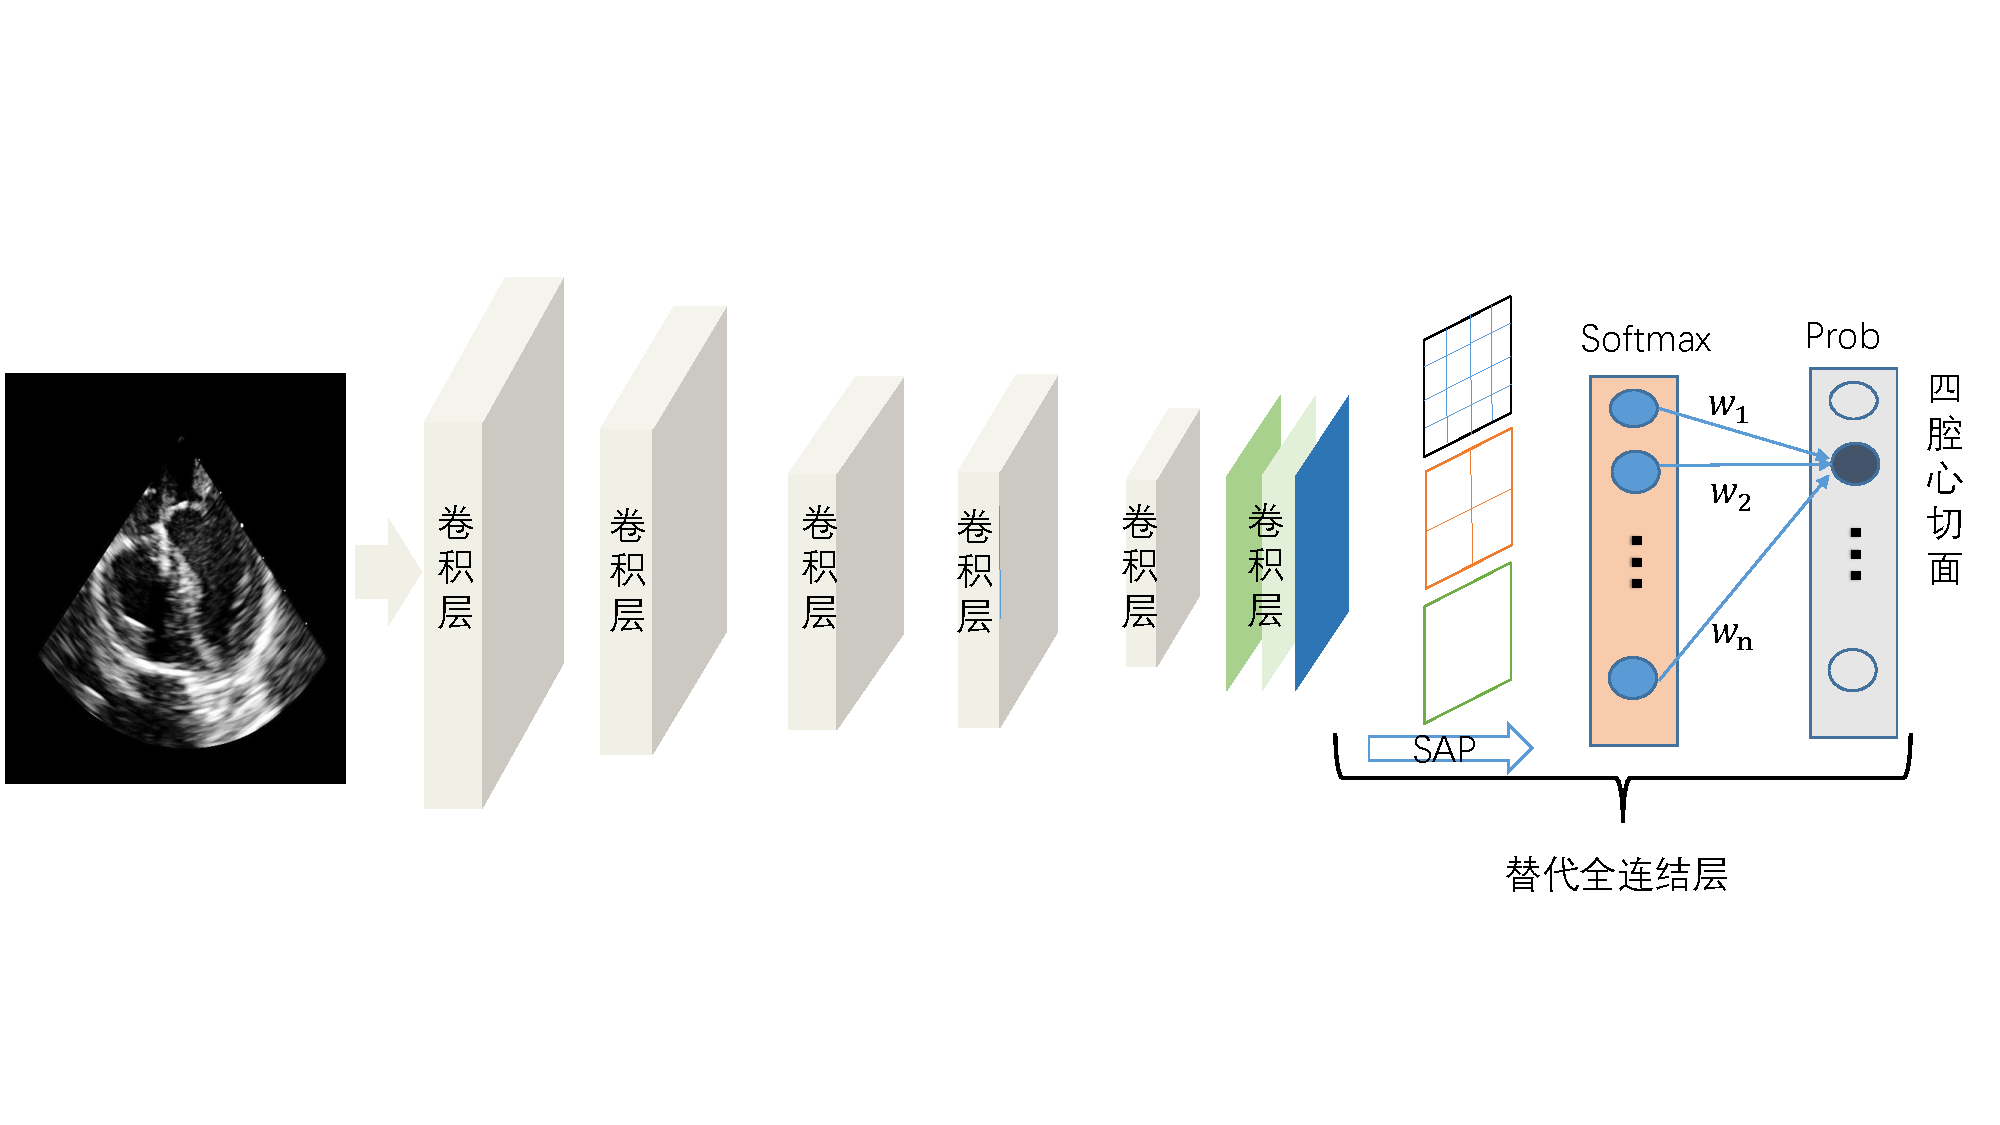
\includegraphics[trim = 30mm 0mm 30mm 0mm, clip, width=0.45\textwidth]{ch03_02}
    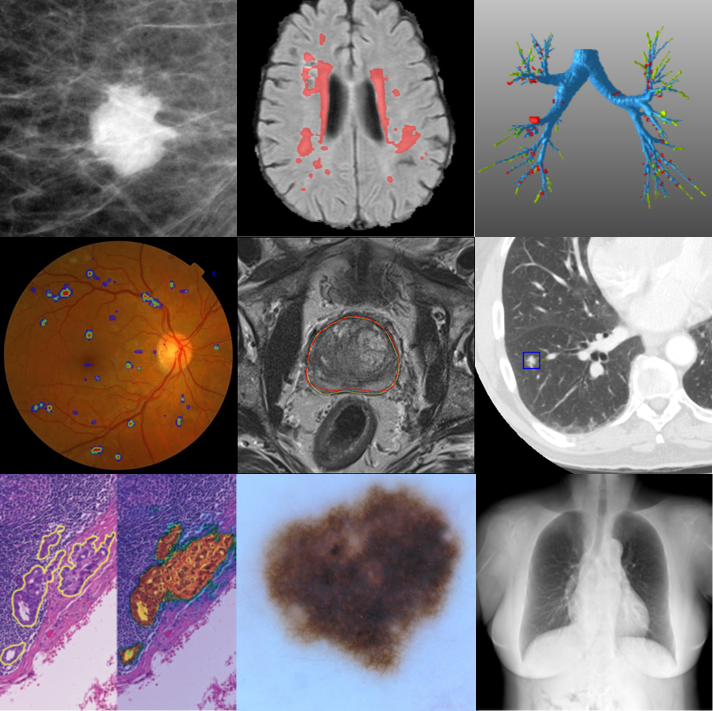
\includegraphics[height=90mm,width=0.9\textwidth]{ch01_05}
   \caption{应用深度学习的一些医学影像图集}
   \label{fig:ch01_05}
\end{figure}

\subsubsection{分类识别}

图像识别分类是深度学习对医学图像分析做出贡献的首要领域之一,尤其是对自然图像进行预训练的CNN已经显示出惊人效果,在一些任务中超过了人类。相关研究表明可以调整CNN以利用医学图像的内在结构,Chen等\citep{Chen2015}利用CNN结合领域知识,在胎儿超声心动图标准切面的自动识别问题中取得良好的识别效果。Bar等\citep{Bar2015Chest}利用自然图像训练的模型对胸腔X-射线图像进行特征提取并结合全局特征\citep{Oliva2001}得到最优检测结果。Margeta等\citep{Margeta2015}针对心脏核磁共振图像利用微调迁移从自然图像学习的模型。总之与自然图像分类相比,医学对象分类较多使用预先训练的网络模型,这主要是缺乏高质量标注的医学数据集,且当前卷积网络较难高效结合上下文或三维信息。

\subsubsection{病变检测} 

CAD在医学图像分析领域是一个非常成熟的任务,解剖对象定位(空间或时间),例如定位器官或标记点,一直是分割任务或制定治疗计划等临床工作流程中的重要预处理步骤。传统CAD\citep{Van2011Computer}通过监督方法或经典的图像处理技术(如滤波和数学形态学)检测候选区域,各阶段通常是分离开的,并常由手工设计的特征来描述,分类器用于将特征向量映射到实际病变的概率。深度学习采用直接以一个以候选病灶为中心的图像数据区域进行操作,训练一个端到端的CNN。如利用深度卷积网络进行显微镜图像中细胞检测\citep{Akram2016}、结合深度全卷积网络的MRI心室检测与分割\citep{Emad2015,Tran2016a}和超声图像解剖结构的检测\citep{Chen2016i}。Roth等人\citep{Roth2016}使用CNN改进三个现有的CAD用于CT结肠镜检查的结肠息肉,体部CT上的硬化性脊柱转移以及体部CT上的肿大淋巴结的检测。
医学成像中的定位通常需要解析3D体积,为了用深度学习算法解决3D数据解析,已经提出了几种将3D空间视为二维正交平面组合的方法,Setio等人\citep{Setio2016Pulmonary}检测在3D胸部CT扫描中的肺结节,使用不同CNN的组合来对每个候选区域进行分类。相关综述请参考文献\citep{Shin2016}。总之与分类识别问题类似,直接解决特定对象检测的问题,需处理如类不平衡、图像的有效像素或体素处理仍是个挑战。

\subsubsection{分割和形状建模}

医学图像中的器官和结构的分割允许定量分析与体积和形状有关的临床参数,它往往是计算机辅助检测的第一步。例如心脏或大脑分中,分割的任务通常被定义为识别组成感兴趣对象的轮廓或内部的体素集。分割是应用医学成像深度学习的论文中最常见的主题,因此也在深度学习方法学中广泛应用,包括开发独特的基于CNN的分割网络结构以及应用循环神经网络(Recurrent Neural Networks,RNNs)进行分割和形状建模。

这些新型CNN架构中最代表性的是由Ronneberger等人\citep{Ronneberger2015}提出的U-Net,将上采样和下采样层的组合,将它们与反卷积和反褶积层之间的所谓跳跃连接相结合,从而直接产生分割图。Milletari等人\citep{Milletari2016}提出了一种称为V-Net的U-Net架构的三维变体。RNN最近在分割任务中变得越来越流行。例如,Xie等人\citep{xie2016}使用空间RNN在组织病理学图像中分割肌束膜。Stollenga等人\citep{cortes2015}首次在6个方向上使用带有卷积层的3D RNNs。此外,基于深度学习的特征点定位方法\citep{Trigeorgis2016}在形状建模方面也取得令人瞩目的结果。总而言之,医学影像的各个细分领域中深度学习相关方法都大量涌入。但一般需直接针对特定分割任务自定义网络结构,相关综述请参考文献\citepns{Zhang2017a}。

\subsubsection{新颖的应用和其他医学分析任务}
\label{sec:applications_various}

在医学图像的配准、基于内容的医学图像检索、图像重建生成和对比增强、融合图像和文本报告、基因组学和医药领域均能找到深度学习的身影,相关综述文献请参考\citepns{Litjens2017Asurvey}。如Kallenberg等\citep{Kallenberg2016Unsupervised}利用无监督的特征学习用于乳房X线照相术,解决乳房密度分割和对乳房X线照片纹理进行风险评分。Yan等\citep{Yan2016Multi}设计了一个多阶段的深度学习回归框架用于图像分类并应用于身体部位识别,它通过多学科的深度学习自动发现了不合理和无信息的局部斑块。苗等人\citep{Miao2016A}提出了一种CNN回归方法,用于实时2-D和3-D配准。Golkov等人\citep{Golkov2016q}提供应用DL将扩散MRI数据处理减少到单个优化步骤,阐明通过使用DNN在逐个体素的基础上的微观结构预测以及健康和损伤组织自动化的无模型分割,展示如何通过深度学习来简化经典数据处理。
\subsubsection{相关软硬件平台}
GPU和GPU计算库(CUDA,OpenCL)的广泛应用促成了深度学习急剧上升的主要原因之一。GPU是高度并行计算引擎,其执行线程数量比中央处理器(CPU)多一个数量级。使用目前的硬件,深度学习GPU的速度通常比CPU快10到30倍。FPGA和定制的深度学习芯片也获得了相当的关注。

除硬件之外,深度学习方法普及的另一推动力是开源软件库和共享深度模型的广泛可用性。这些库提供了神经网络中重要操作(如卷积、循环网络)的高效GPU实现方便用户使用。当前流行的软件包是(按字母顺序):
\begin{itemize}
 \item {\bf Caffe} \citep{Jia2014}. 提供C ++和Python接口,由加州大学伯克利分校的研究生开发。
 \item {\bf Tensorflow} \citep{Abadi2016TensorFlow}. 由Google开发提供C ++,Python和接口.
 \item {\bf Theano} \citep{AlRfou2016Theano}. 提供由蒙特利尔MILA实验室开发的Python库。
 \item {\bf Mxnet} \citep{Chen2015mxnet}. 提供一个python和C++接口,是亚马逊的云平台默认深度学习引擎  
\end{itemize}
 
\subsubsection{趋势及挑战}

深度学习已经渗透到医学影像分析的各个方面,深度学习在医学图像分析中的应用文献首先出现在各种研讨会和会议上(MICCAI,SPIE,ISBI和EMBC等),然后在期刊中出现。该主题现已在主要会议和医学影像分析期刊中占据主导地位。收益于深度学习算法的突破以及现代GPU高效并行计算能力的提升,引起了巨大的商业兴趣。通用电气,西门子和飞利浦都将深度学习算法整合到成像设备和图像处理系统中以加速自动化定位分割解剖结构,以大大加快工作流程并消除了互操作性差异的问题,或执行自动量化。诸多创业医学影像公司,比如美国的Enlitic和国内的DeepCare,同样使用AI快速筛选海量大数据,或者提供即时的临床决策支持。

将深度学习算法应用于医学图像分析面临许多独特的挑战。针对数据的主要挑战不仅是影像数据本身(数据维度和隐私等问题)的可用性,还要获取这些影像的相关注释/标签,也需要考虑通过众包来利用非专家标签减少对专家经验的需求;训练深度学习系统需要仔细考虑如何处理图像中的噪声和不确定性,类别不平衡问题特别严重;能否从一般图像向相关医学领域迁移学习;另一个挑战是平衡深度学习网络中的特征的数量(通常是数千个)与临床特征的数量(通常只有少数)以防止临床特征被淹没; 

多数文献都集中在有监督的深度学习方法上以实现分类,检测,分割和标注等。然而应用无监督深度学习的兴趣仍在,并最近又重新开始收到重视,主要是因为世界上可用的大多是未标记数据;并且人类学习在一定程度上以无监督的方式发生,远比监督学习方法高效,如何在不知道具体标签的情况下学会识别物体和结构,或者如何只需要非常有限的监督就可以将这些对象分类。

最后,深度学习方法缺乏理论分析,经常被认为是“黑匣子”。尤其在医学领域可解释性尤其重要,算法系统必须能够以某种方式进行自我评估。这是将深度学习方法应用于医学图像分析,加速临床医生和患者对深度学习应用的接受程度的关键所在。

\section{创新点及全文结构}

所在的研究组多年来与四川大学华西医院合作展开医学影像处理系统中关键技术的研究。博士期间在相关课题资助下,关注于深度学习和医学影像学,着重于机器学习及其在医学影像领域的作用。本文在深度学习理论层面讨论了深度可视化问题,报告了我们在基于深度学习架构的经食道超声心动图标准切面自动分类识别,对一般医学组织对象的定位检测和对超声心动图左心室分割三个主要部分进行研究。

主要研究内容及成果如下:

1)应用深度学习进行医学图像的分类识别,通过构建超声心动图标准切面数据库,提出了一种基于深度卷积神经网络的超声心动图标准切面自动识别方法,该算法针对网络全连接层占有模型大部分参数的缺点,引入空间金字塔均值池化替代全连接层,获得更多的空间结构信息,利用全局空间金字塔均值池化方法进行微调迁移学习,并大大减少模型参数、降低过拟合风险,通过类别显著性区域将类似注意力机制引入模型可视化过程,详尽分析了数据规模对模型分类精度的影响,并对模型的可解释性和有效性进行了分析。

2)针对基于深度卷积神经网络的图像分类模型的可解释性问题,通过评估模型特征空间的潜在可表示性,提出一种用于改善理解模型特征空间的可视化方法。给定任何已训练的深度卷积网络模型,引入了通过激活最大化获得的图像可解释性的正则化方法,结合现有正则化方法提出空间金字塔分解方法,利用构建多层拉普拉斯金字塔主动提升目标图像特征空间的低频分量,结合多层高斯金字塔调整其特征空间的高频分量得到较优可视化效果。并通过限制可视化区域,提出利用类别显著性激活图技术加以压制上下文无关信息,可进一步改善可视化效果。该模型有效克服了原有可视化方法中由于不能主动调整高低频分量等原因造成的可视化图像语义重复和低效率等问题。

3)针对自动检测医学图像中指定目标时存在的问题,提出了一种基于深度学习自动检测目标位置和估计对象姿态的算法。该算法基于区域深度卷积神经网络和目标结构的先验知识,采用区域生成候选框网络、感兴趣区域池化策略,引入包括分类损失、边框位置回归定位损失和像平面内朝向损失的多任务损失函数,近似优化一个端到端的有监督定位网络,能快速地对医学图像中目标自动定位,有效地为下一步的分割和参数自动提取提供定位结果。并在超声心动图左心室检测中提出利用检测额外标记点:二尖瓣环、心内膜垫和心尖,能高效地对左心室朝向姿态进行估计。

4)针对图像内容理解的底层任务,图像去噪和分割分别设计利用了全卷积网络,针对不同的具体任务设计损失函数,提出了一个有监督多层残差卷积网络框架,结合不同损失函数学习端到端映射变换应用于去躁和心室图像的分割;其中分割任务是设计了不同架构的单通道CNNs分割模型,与如今流行的分割方法比较,大大提高了分割与识别正确率。


\section{论文的章节安排}

全篇共八章,结构如下:

第一章绪论介绍了应用人工智能进行医学影像分析的研究背景及意义,对当前国内外的研究现状及挑战进行剖析,同时阐述了本论文的研究内容,列出了主要创新点,最后给出了整篇文章的章节安排。

第二章概述了用于医学影像分析的主要深度学习算法和描述了统计形状模型。在这章中简述了各种神经网络,分析网络结构、优化算法和训练中的关键技术;接着介绍了传统的医学图像分割算法中的统计形变模型。

第三章描述了本文的基于CNNs的超声心动图标准切面识别方法。该章首先描述了传统CNNs算法应用于医学图像中存在的不足;然后提出了一种综全局空间信息的卷积神经网络模型,并可视化分析了模型的有效性;实验结果表明本章方法优于传统CNNs模型。

第四章介绍了本文提出的空间金字塔分解的深度可视化算法。首先描述了传统深度可视化方法存在的问题;然后介绍了基于梯度更新的可视化方法;接着提出了利用空间金字塔分解主动调整高低频分量;最后实验验证了本文方法的鲁棒性。

第五章分析了本文提出的基于区域卷积神经网络的心室检测算法。首先,分析了检测算法的形式化定义,概述了物体检测的演进;之后列出了对候选区域生成网络的改进检测物体朝向;并结合带朝向的多任务损失函数进行困难样例挖掘;然后详细从MRI及超声二维数据全面验证本文检测方法的有效性和鲁棒性。

第六章分析了本文提出的基于Encoder-Decoder 网络的去躁算法。首先,分析了本章算法的相关工作;之后列出了提出方法的主要内容;最后实验验证了提出方法的有效性;介绍了基于卷积神经网络的形状对齐算法。首先,指出初始位置定位和特征点标注方法,即要解决定位检测问题;之后列出了如何结合卷积神经网络特征的AAM模型与CLM模型;然后详细介绍了基于不同特征的分割结果。

最后总结全文,并展望了未来的研究工作。